%!TEX root = ../main.tex
%
% 波の性質
%


\section{波の性質}

\subsection{「波」とは}

\subsubsection*{私たちの身の周りにある波}

\begin{center}
\begin{tabular}{ccl}
水面(海面や湖面)に立つ波 & $\Rightarrow$ & 目で形を見ることができる波\\
サイレンなどの音の波(音波) &  $\Rightarrow$ & 耳で聞くことのできる波\\
地震波 & $\Rightarrow$ & 身体で感じることができる波
\end{tabular}
\end{center}

これらは、振動が水、空気などの媒質の中を伝わっていく現象で、この振動は、
\begin{center}
\begin{tabular}{lcl}
波長 &:&$\lambda$(ラムダ)\\
振動数(周波数)&:&$\nu$(ニュー)\\
振幅&:&$A$\\
\end{tabular}
\end{center}
によって表わされます。この場合の波の伝わる速度$v$は、
\begin{center}
波の伝わる速度:$v=\lambda \nu$
\end{center}
です。また、振動数(周波数)と「波が1波長進むのにかかる時間」=周期とは互いに逆数の関係があり、
\begin{center}
周期:$T=\frac{1}{\nu}$
\end{center}
となります。
\begin{center}
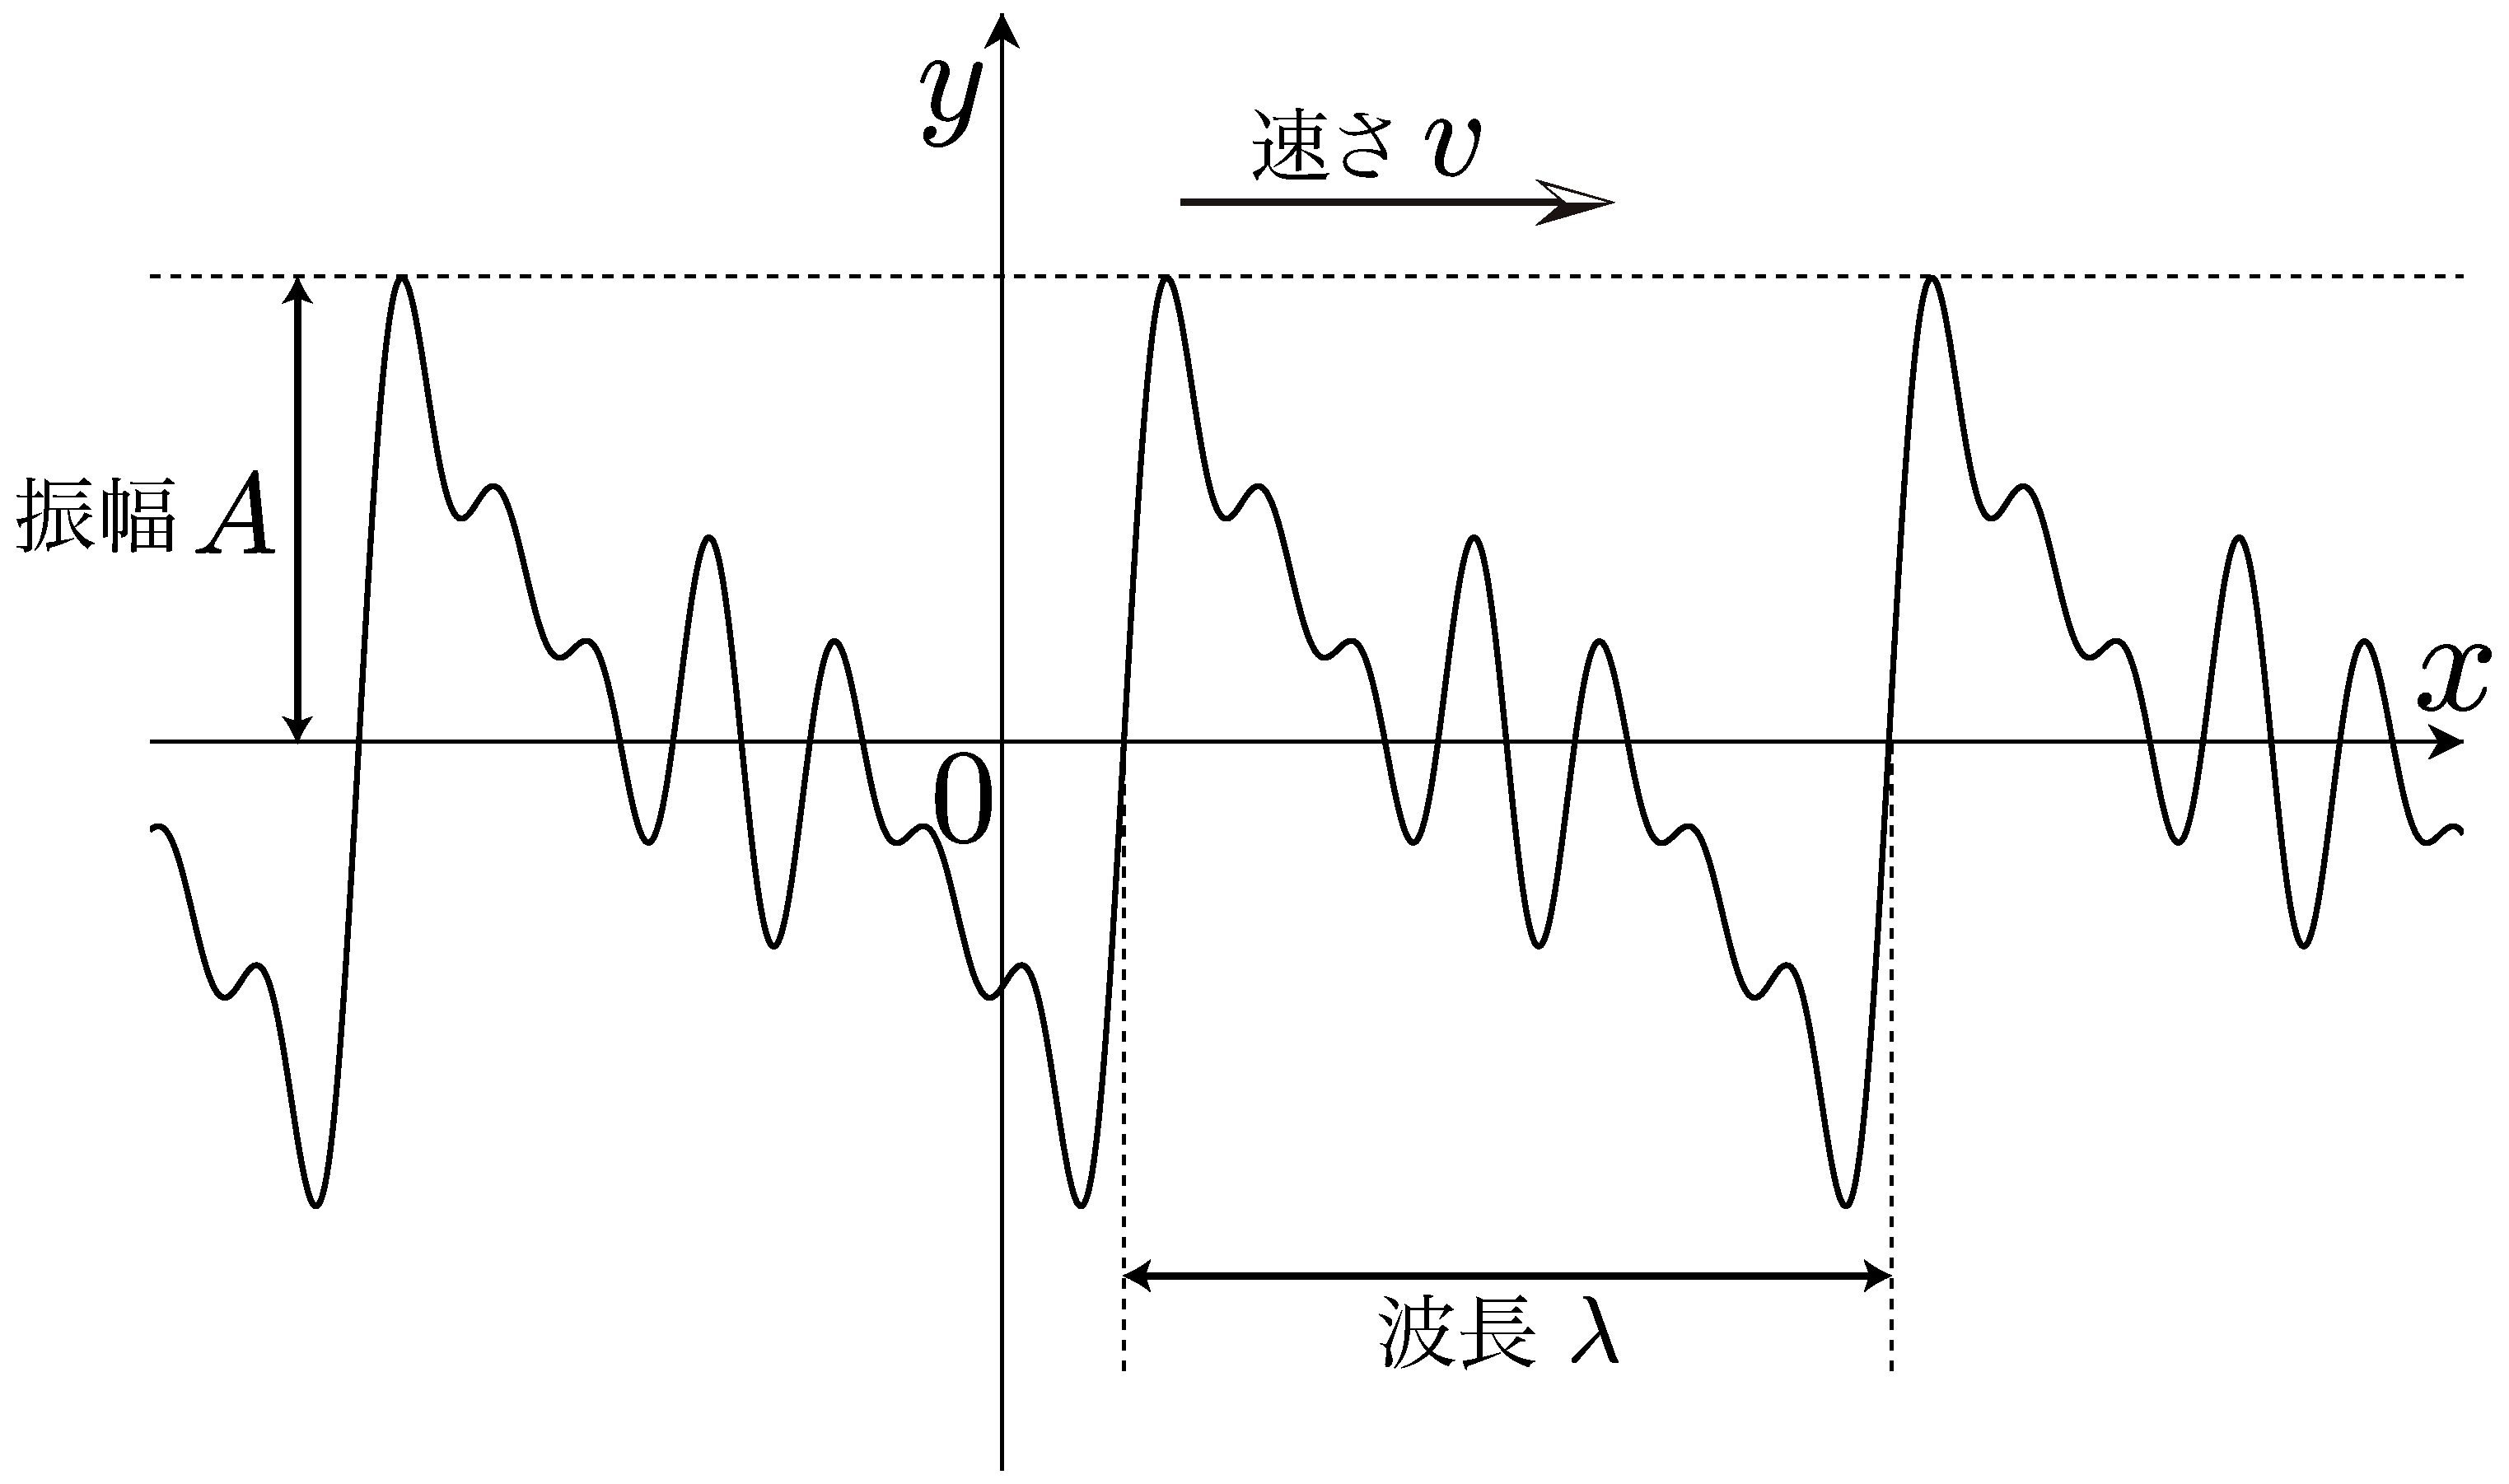
\includegraphics[scale=0.18]{01_Wave/wave1.eps}
\end{center}

波の基本の形は次のような正弦波(サイン関数で表わされる波)で、変位$y$は、時間$t$と位置$x$の関数で表わされます。
\[
y = A \sin\left(2\pi \left(\frac{t}{T}-\frac{x}{\lambda}\right)\right)
\]
ここで、式中の$\pi$は円周率=$3.1415\ldots$です。
\begin{center}
\begin{tabular}{ccc}
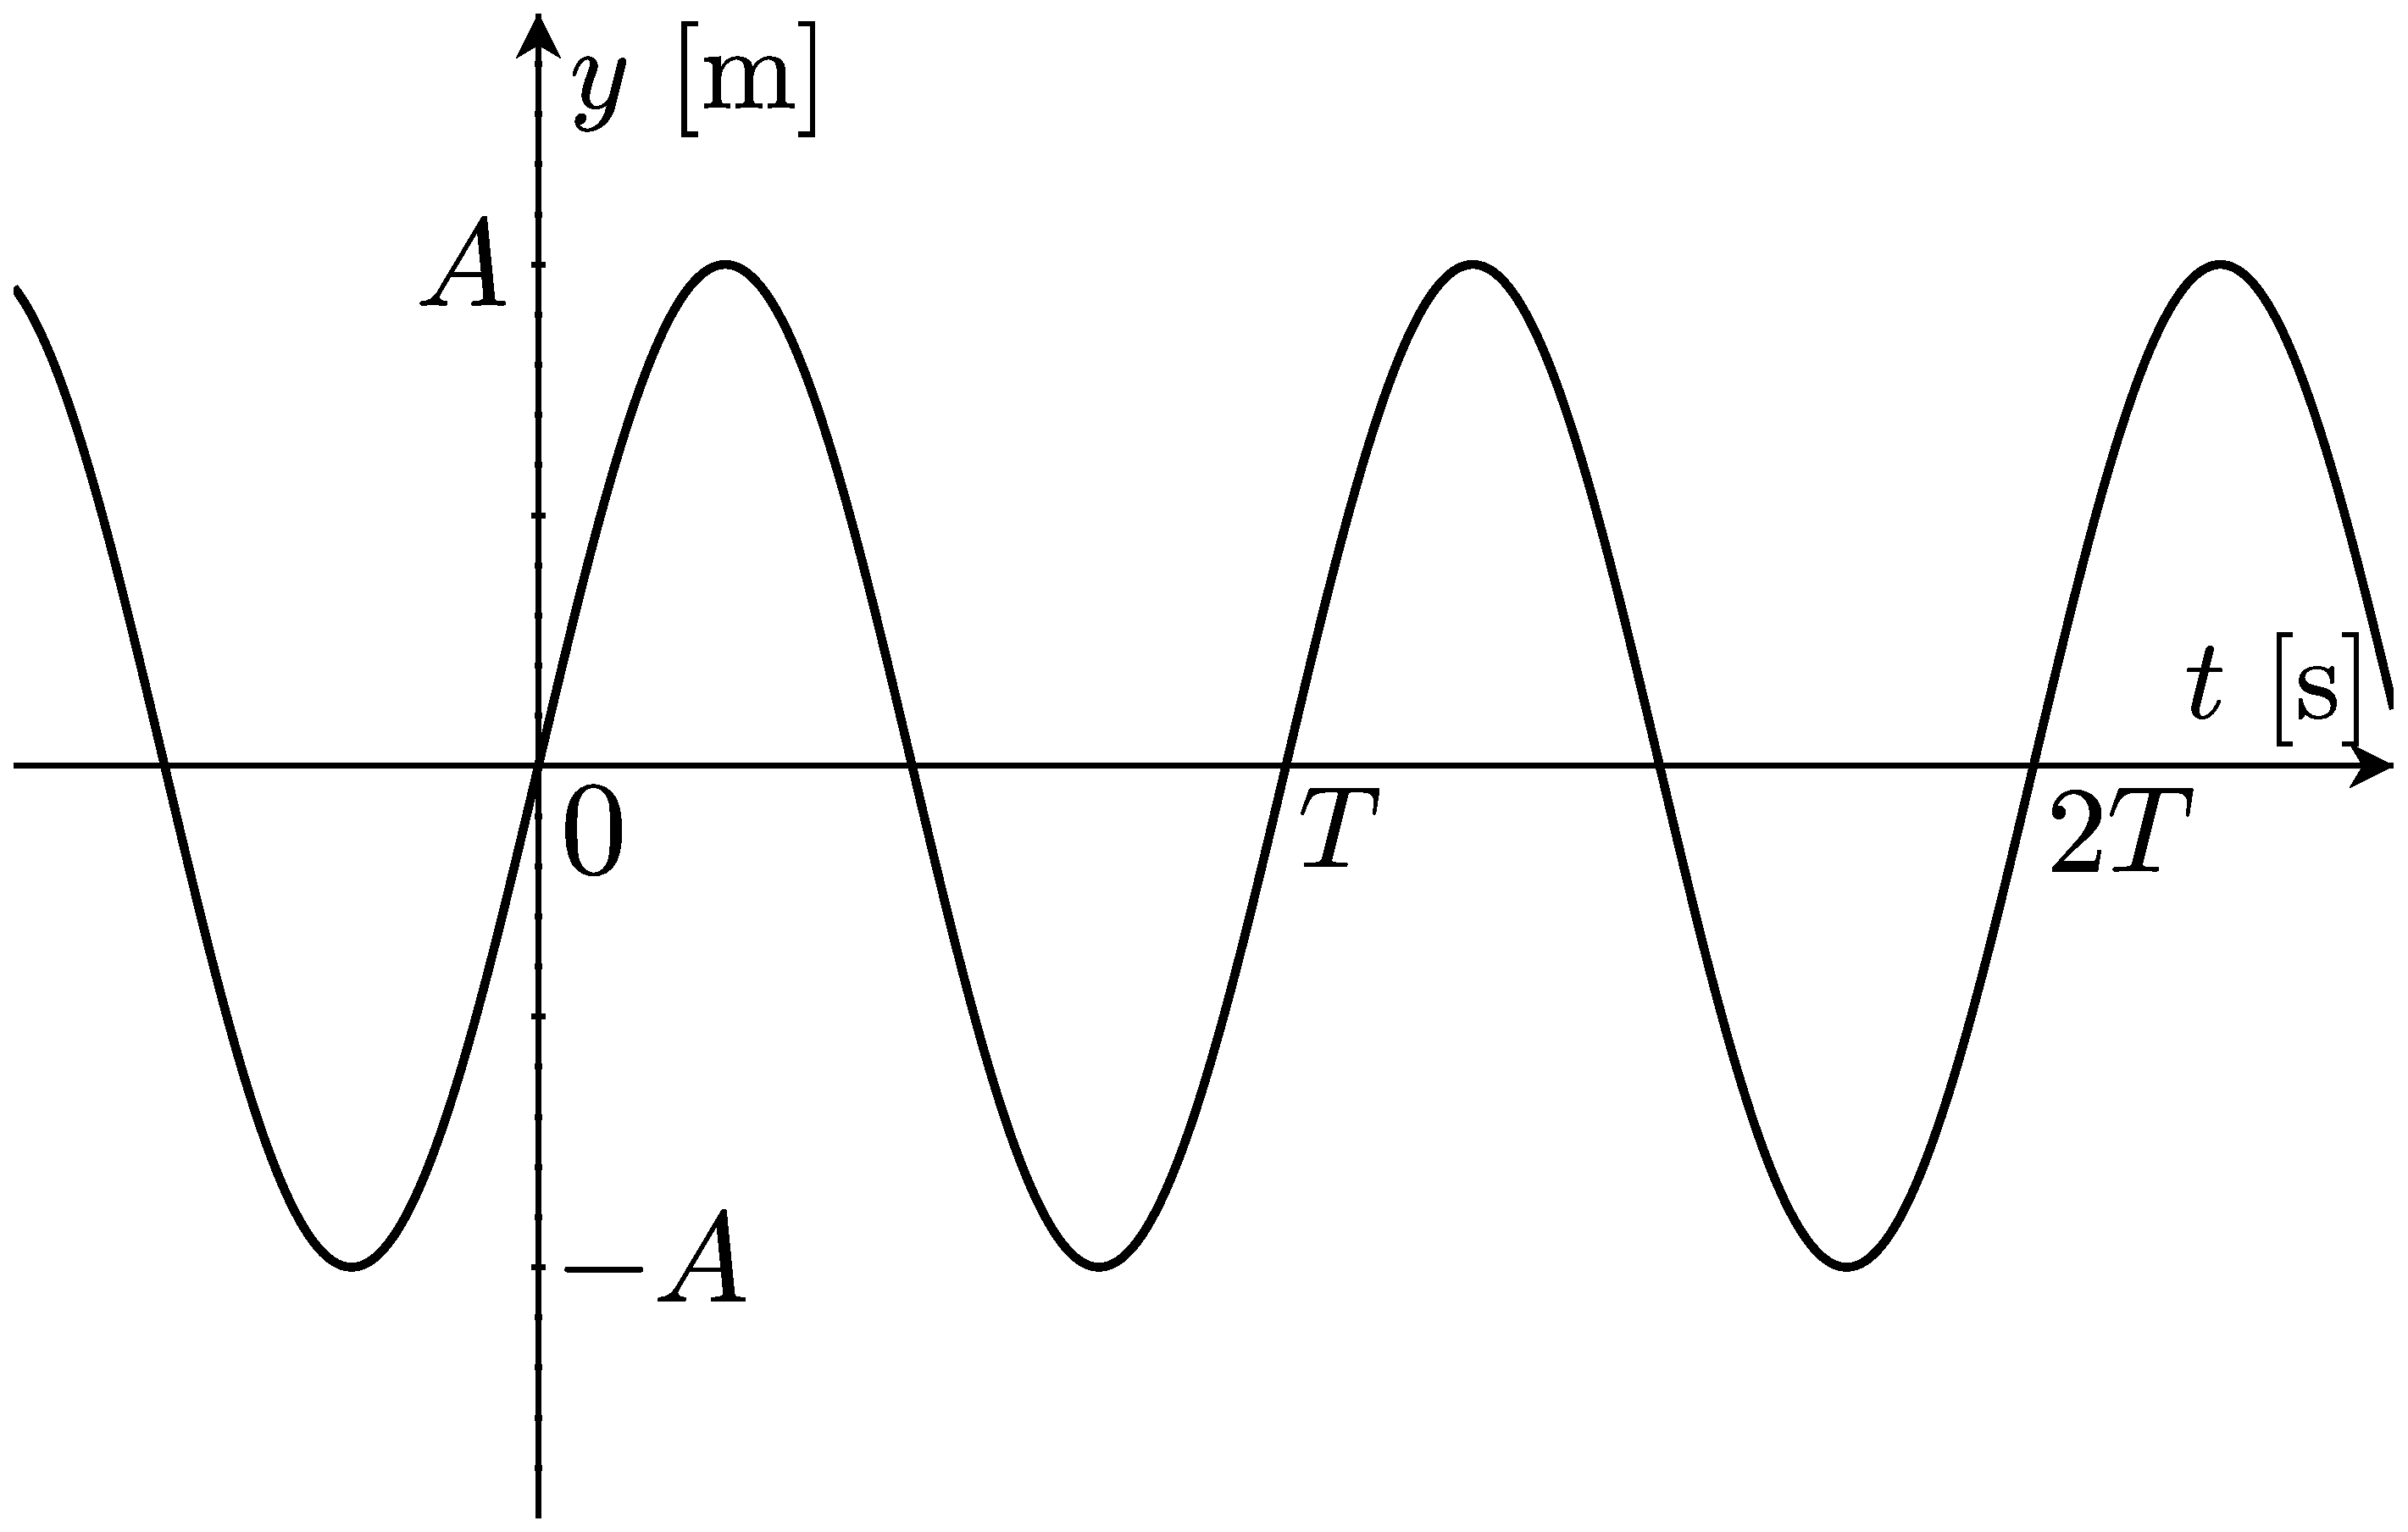
\includegraphics[scale=0.14]{01_Wave/wave2.eps}&&
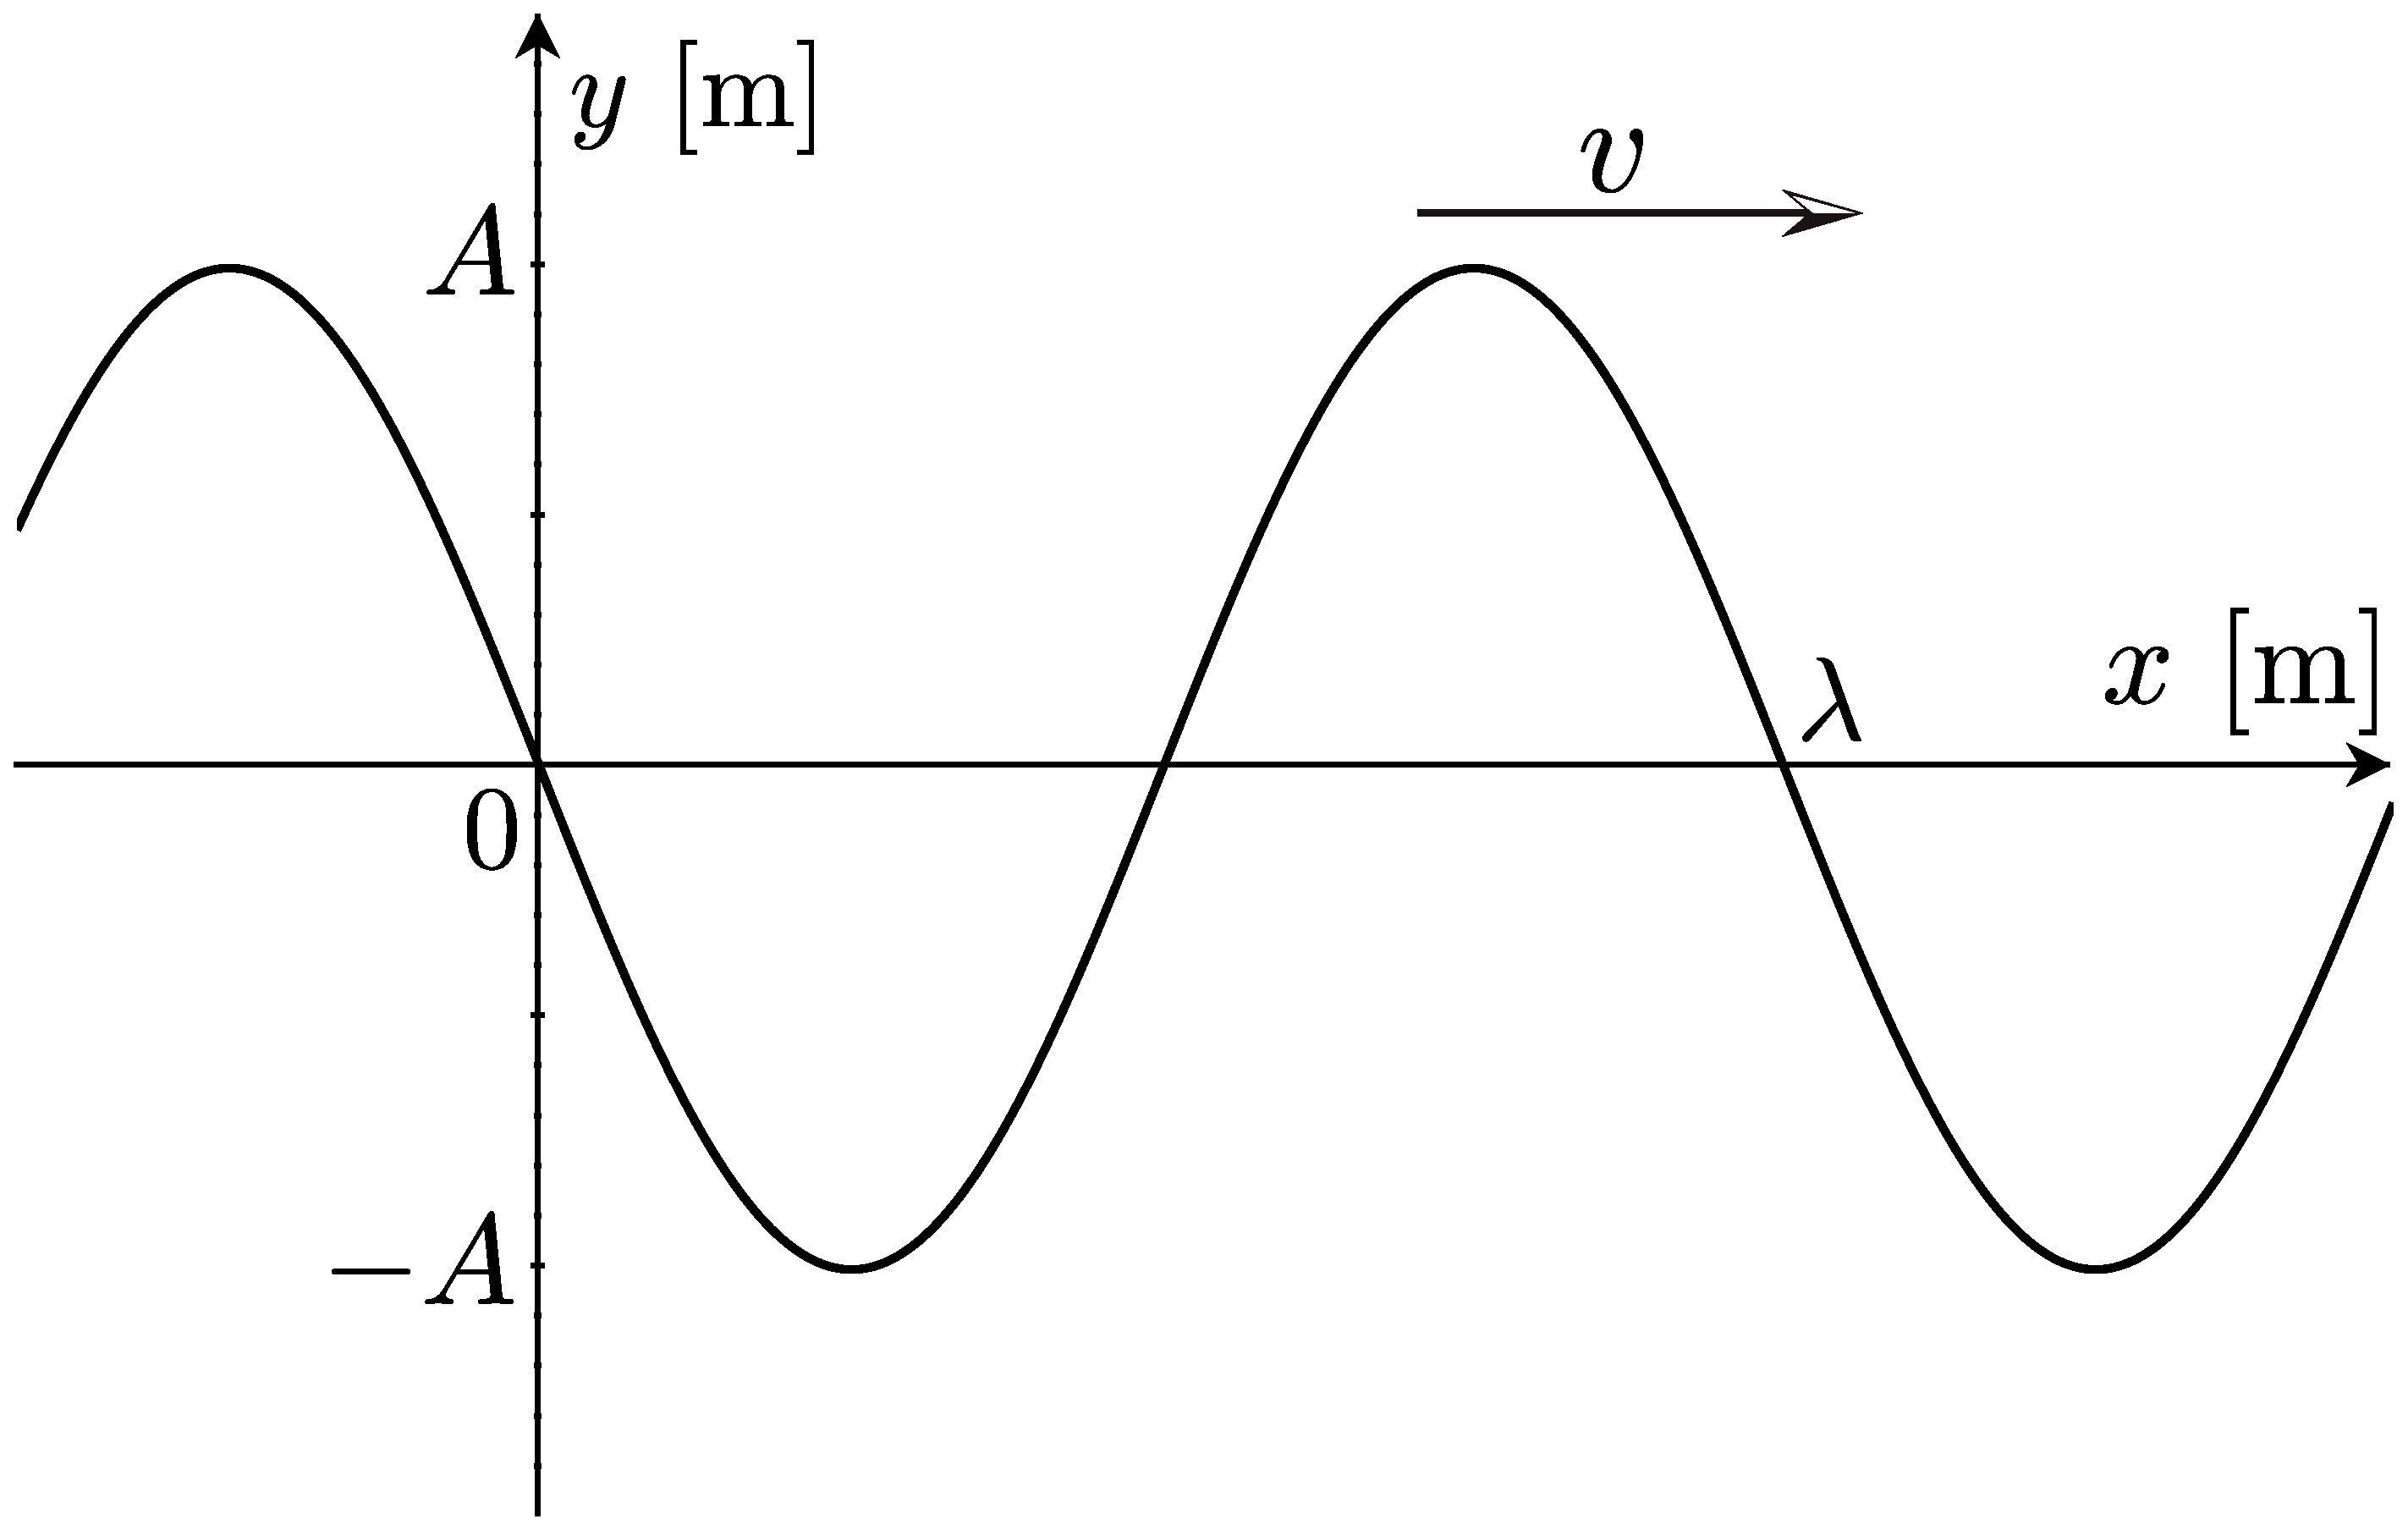
\includegraphics[scale=0.14]{01_Wave/wave3.eps}\\
(a) $x=0$の点の振動のグラフ && (b) $t=0$のときの波のグラフ\\
\end{tabular}
\end{center}



%\subsubsection*{波の性質と種類}

\begin{itemize}

\item 波には、{\bf 屈折}、{\bf 反射}、{\bf 回折}、{\bf 干渉}などの性質があります。

\item 波の振動の伝わり方によって種類が分けられています。
\begin{center}
\begin{tabular}{rcl}
{\bf 横波} &$\cdots$& 波の振動方向が、波の進行方向に対して垂直のもの\\
&& 例)水面の波、地震のS波\\
{\bf 縦波} & $\cdots$ &波の振動方向が、波の進行方向と同じもの\\
&& 例)音波、地震のP波
\end{tabular}
\end{center}

\end{itemize}


\subsection{波の干渉と回折}

\subsubsection{波の位相と干渉}


波の1周期における波形の位置のことを位相といい、1周期を360度=$2\pi$として角度で 
表します。すなわち、波の基本形の式
$y=A\sin\left(2\pi\left(\frac{t}{T}-\frac{x}{\lambda}\right)\right)$
において、 
$
2\pi\left(\frac{t}{T}-\frac{x}{\lambda}\right)
$
が位相で、 
$
\frac{t}{T}
$
は時間という物差しで時間$t$の中に波がいくつ入るかを、
$\frac{x}{\lambda}$は長さで見て距離$x$の中に波がいくつ入るかを数えています。

波の重ね合わせの原理により、同位置同時刻において位相が同じである2つの波は強め合い、位相がちょうど「半周期分=180度」ずれている波は弱め合います。
このような波の性質を{\bf 干渉}といいます。

\begin{center}
\begin{tabular}{ccc}
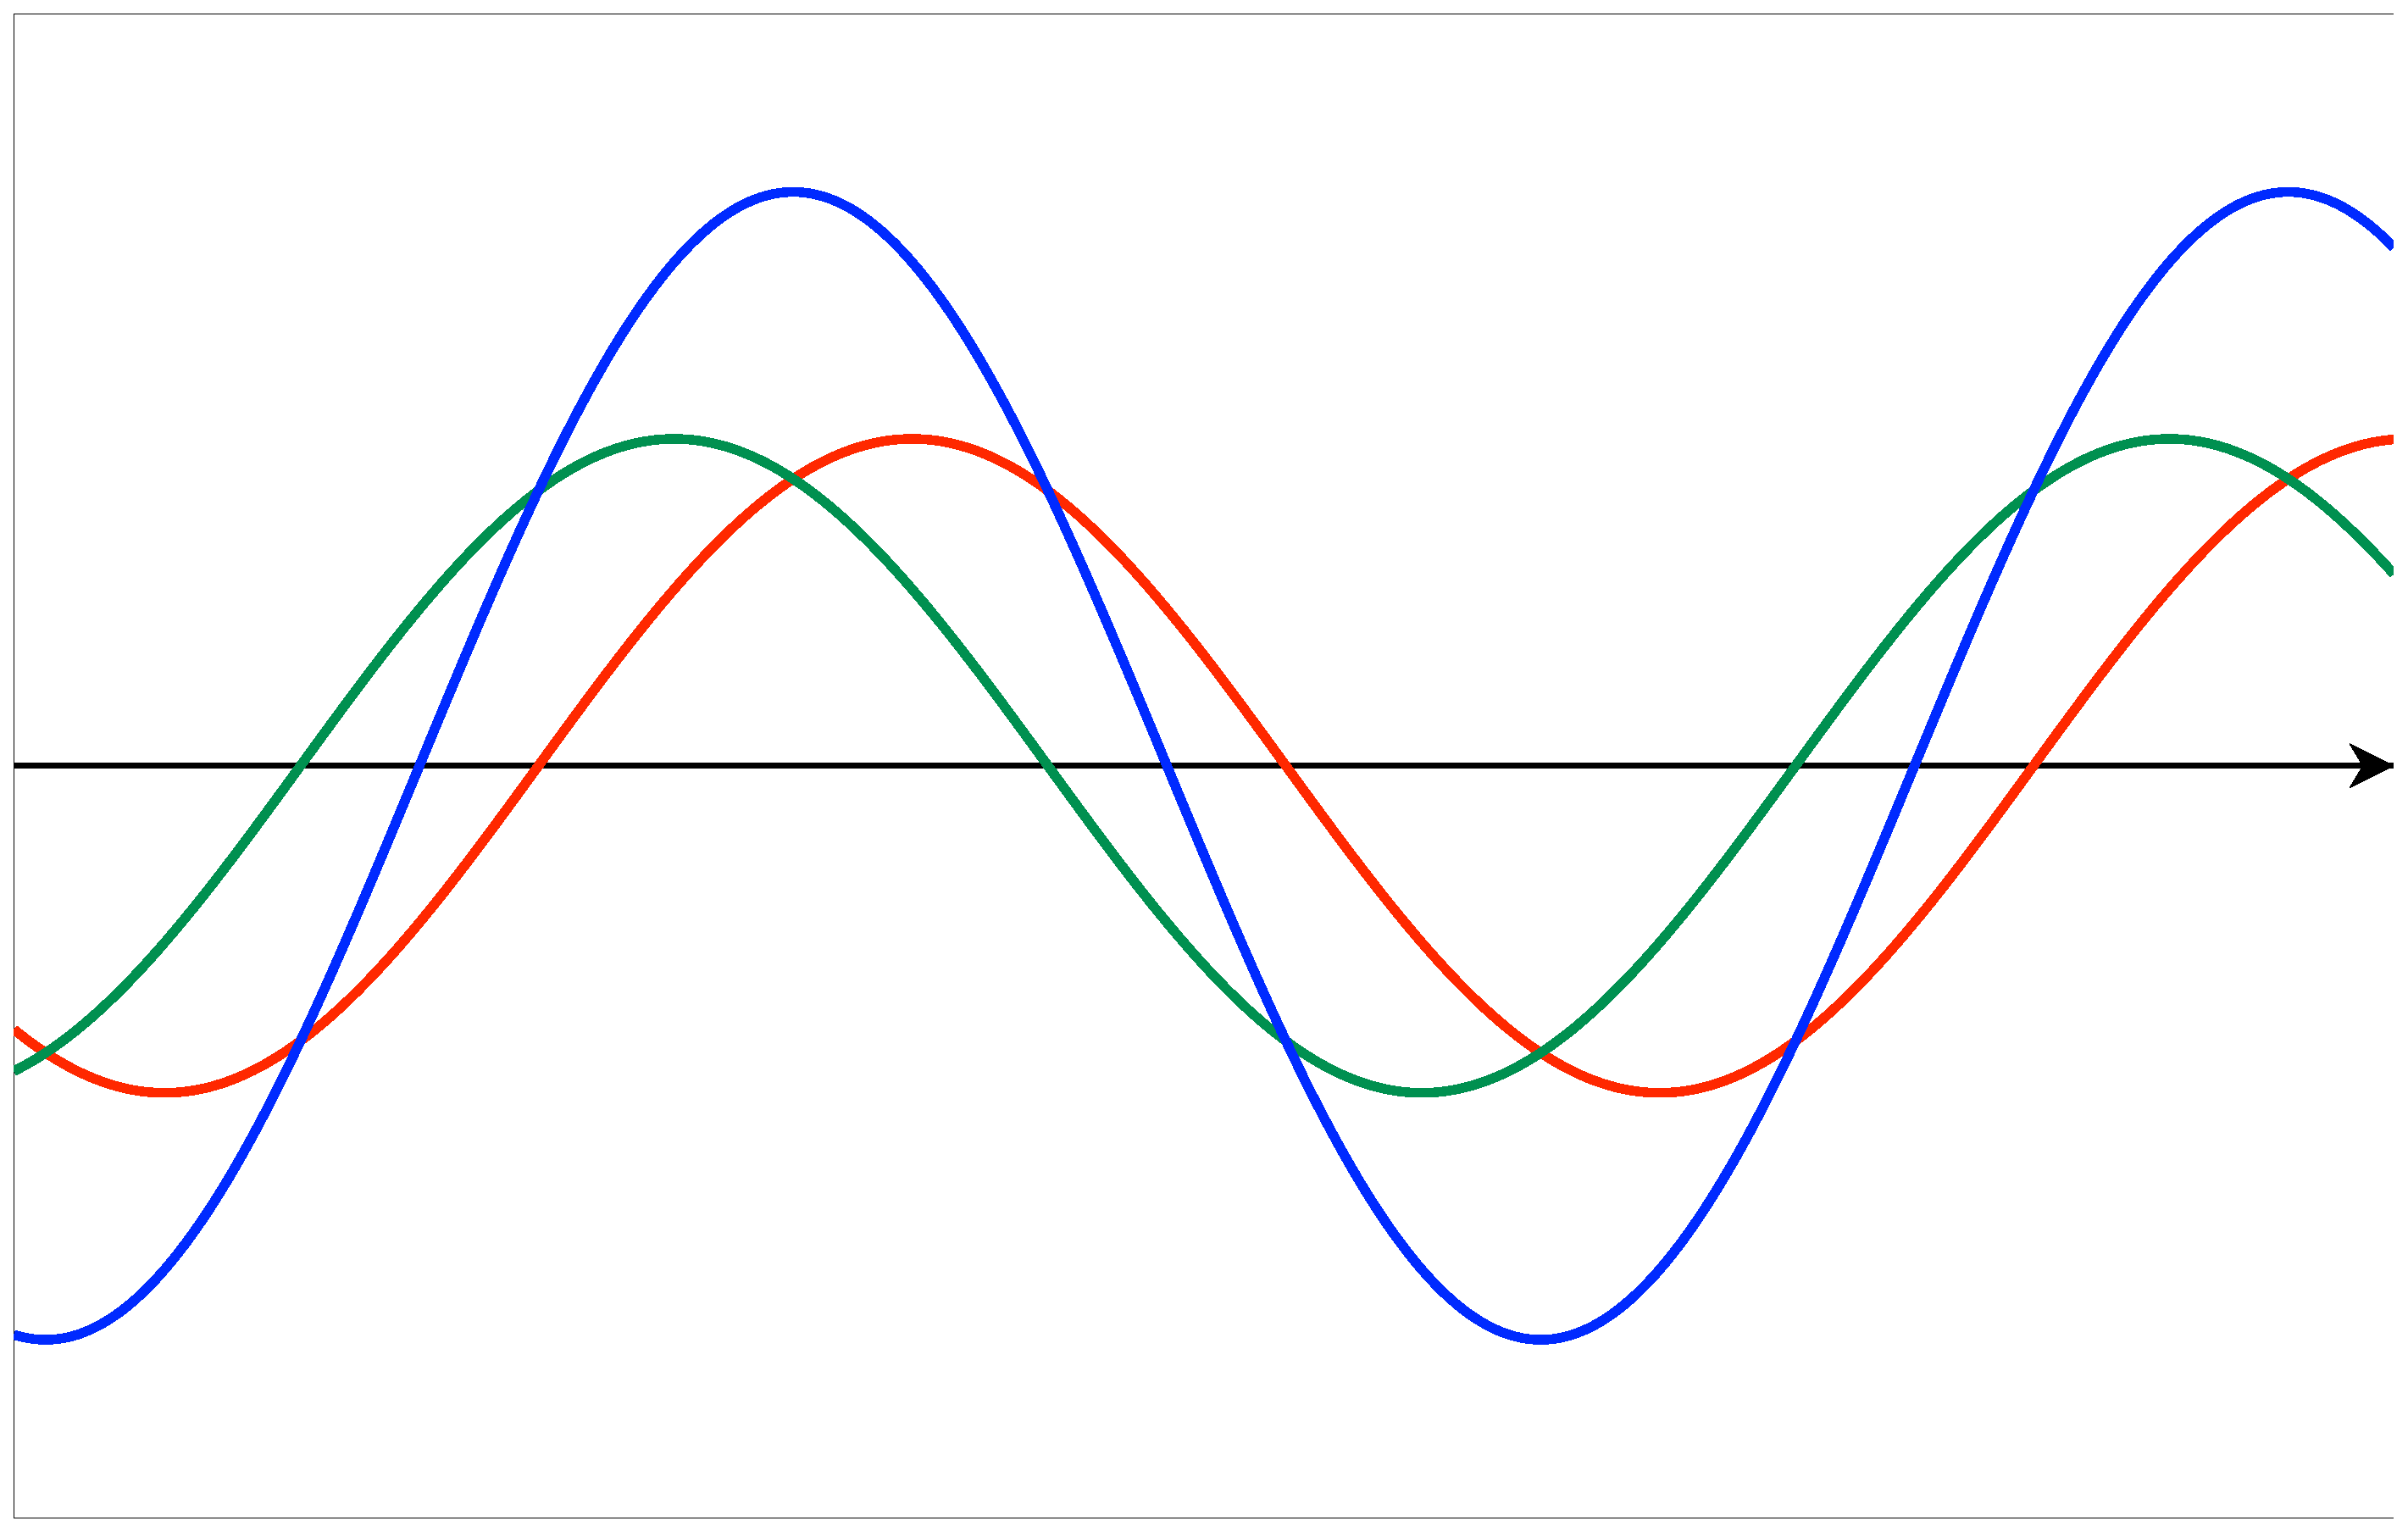
\includegraphics[scale=0.1]{01_Wave/interference1.eps}&
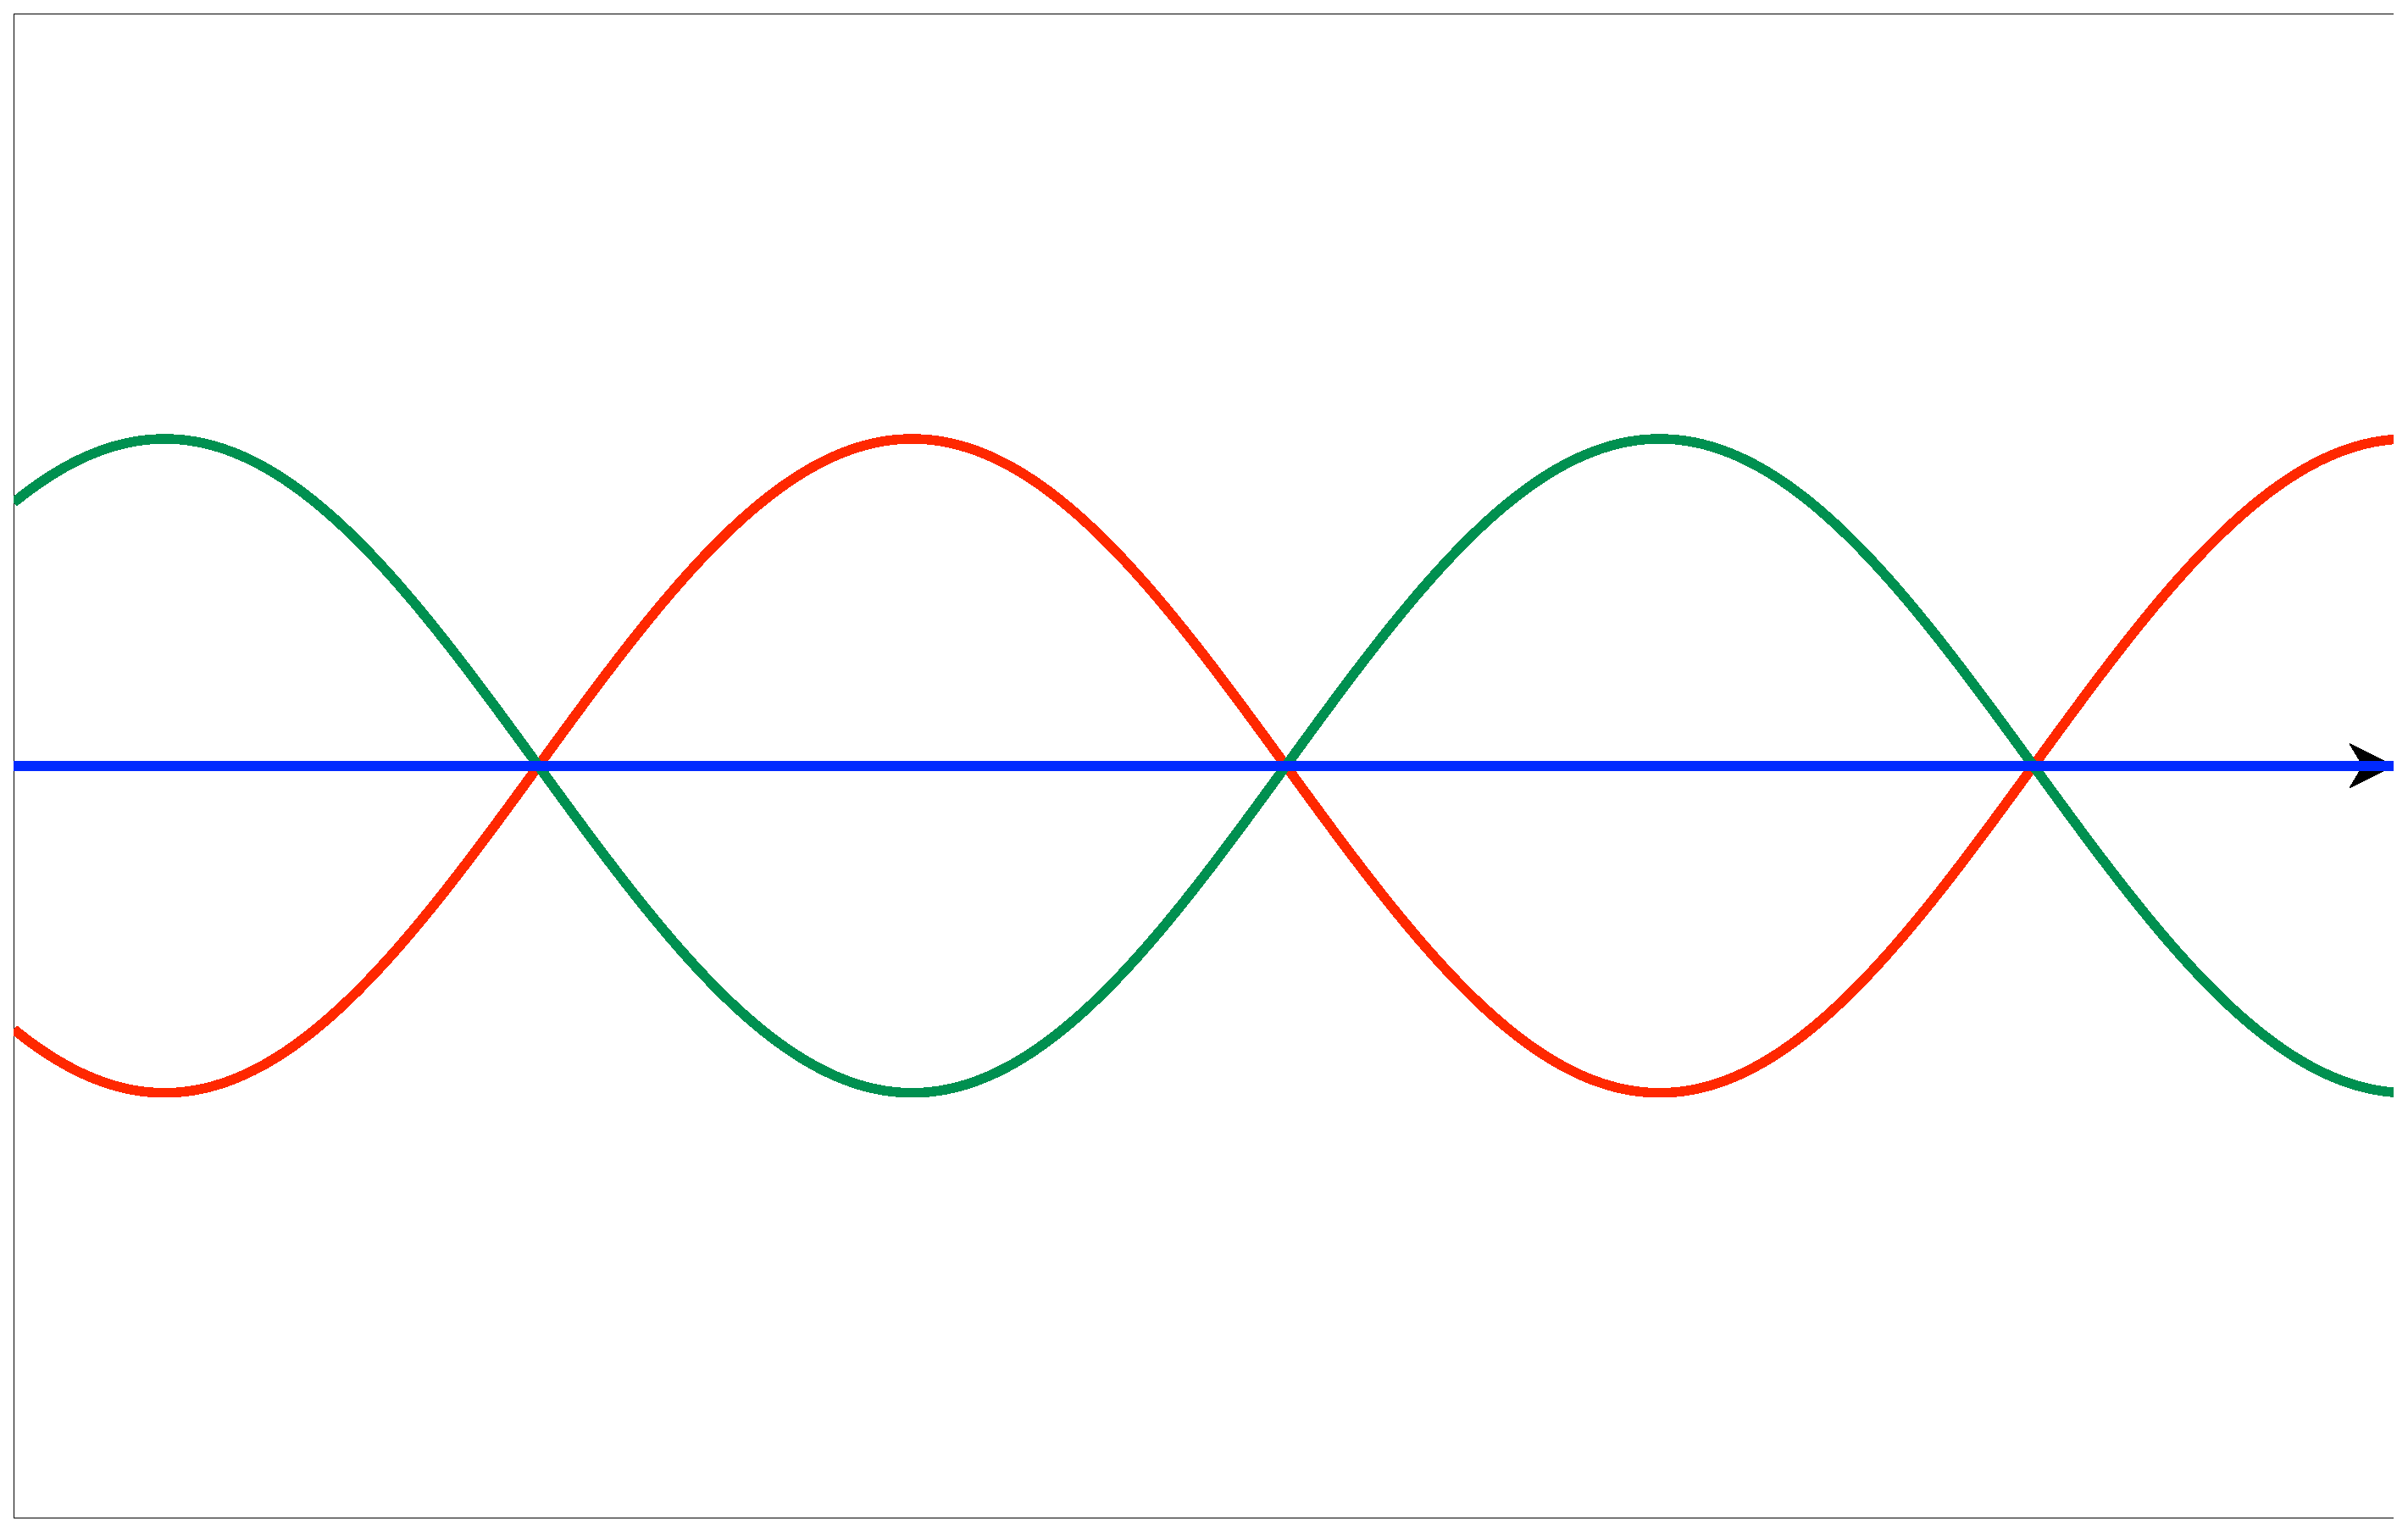
\includegraphics[scale=0.1]{01_Wave/interference2.eps}&
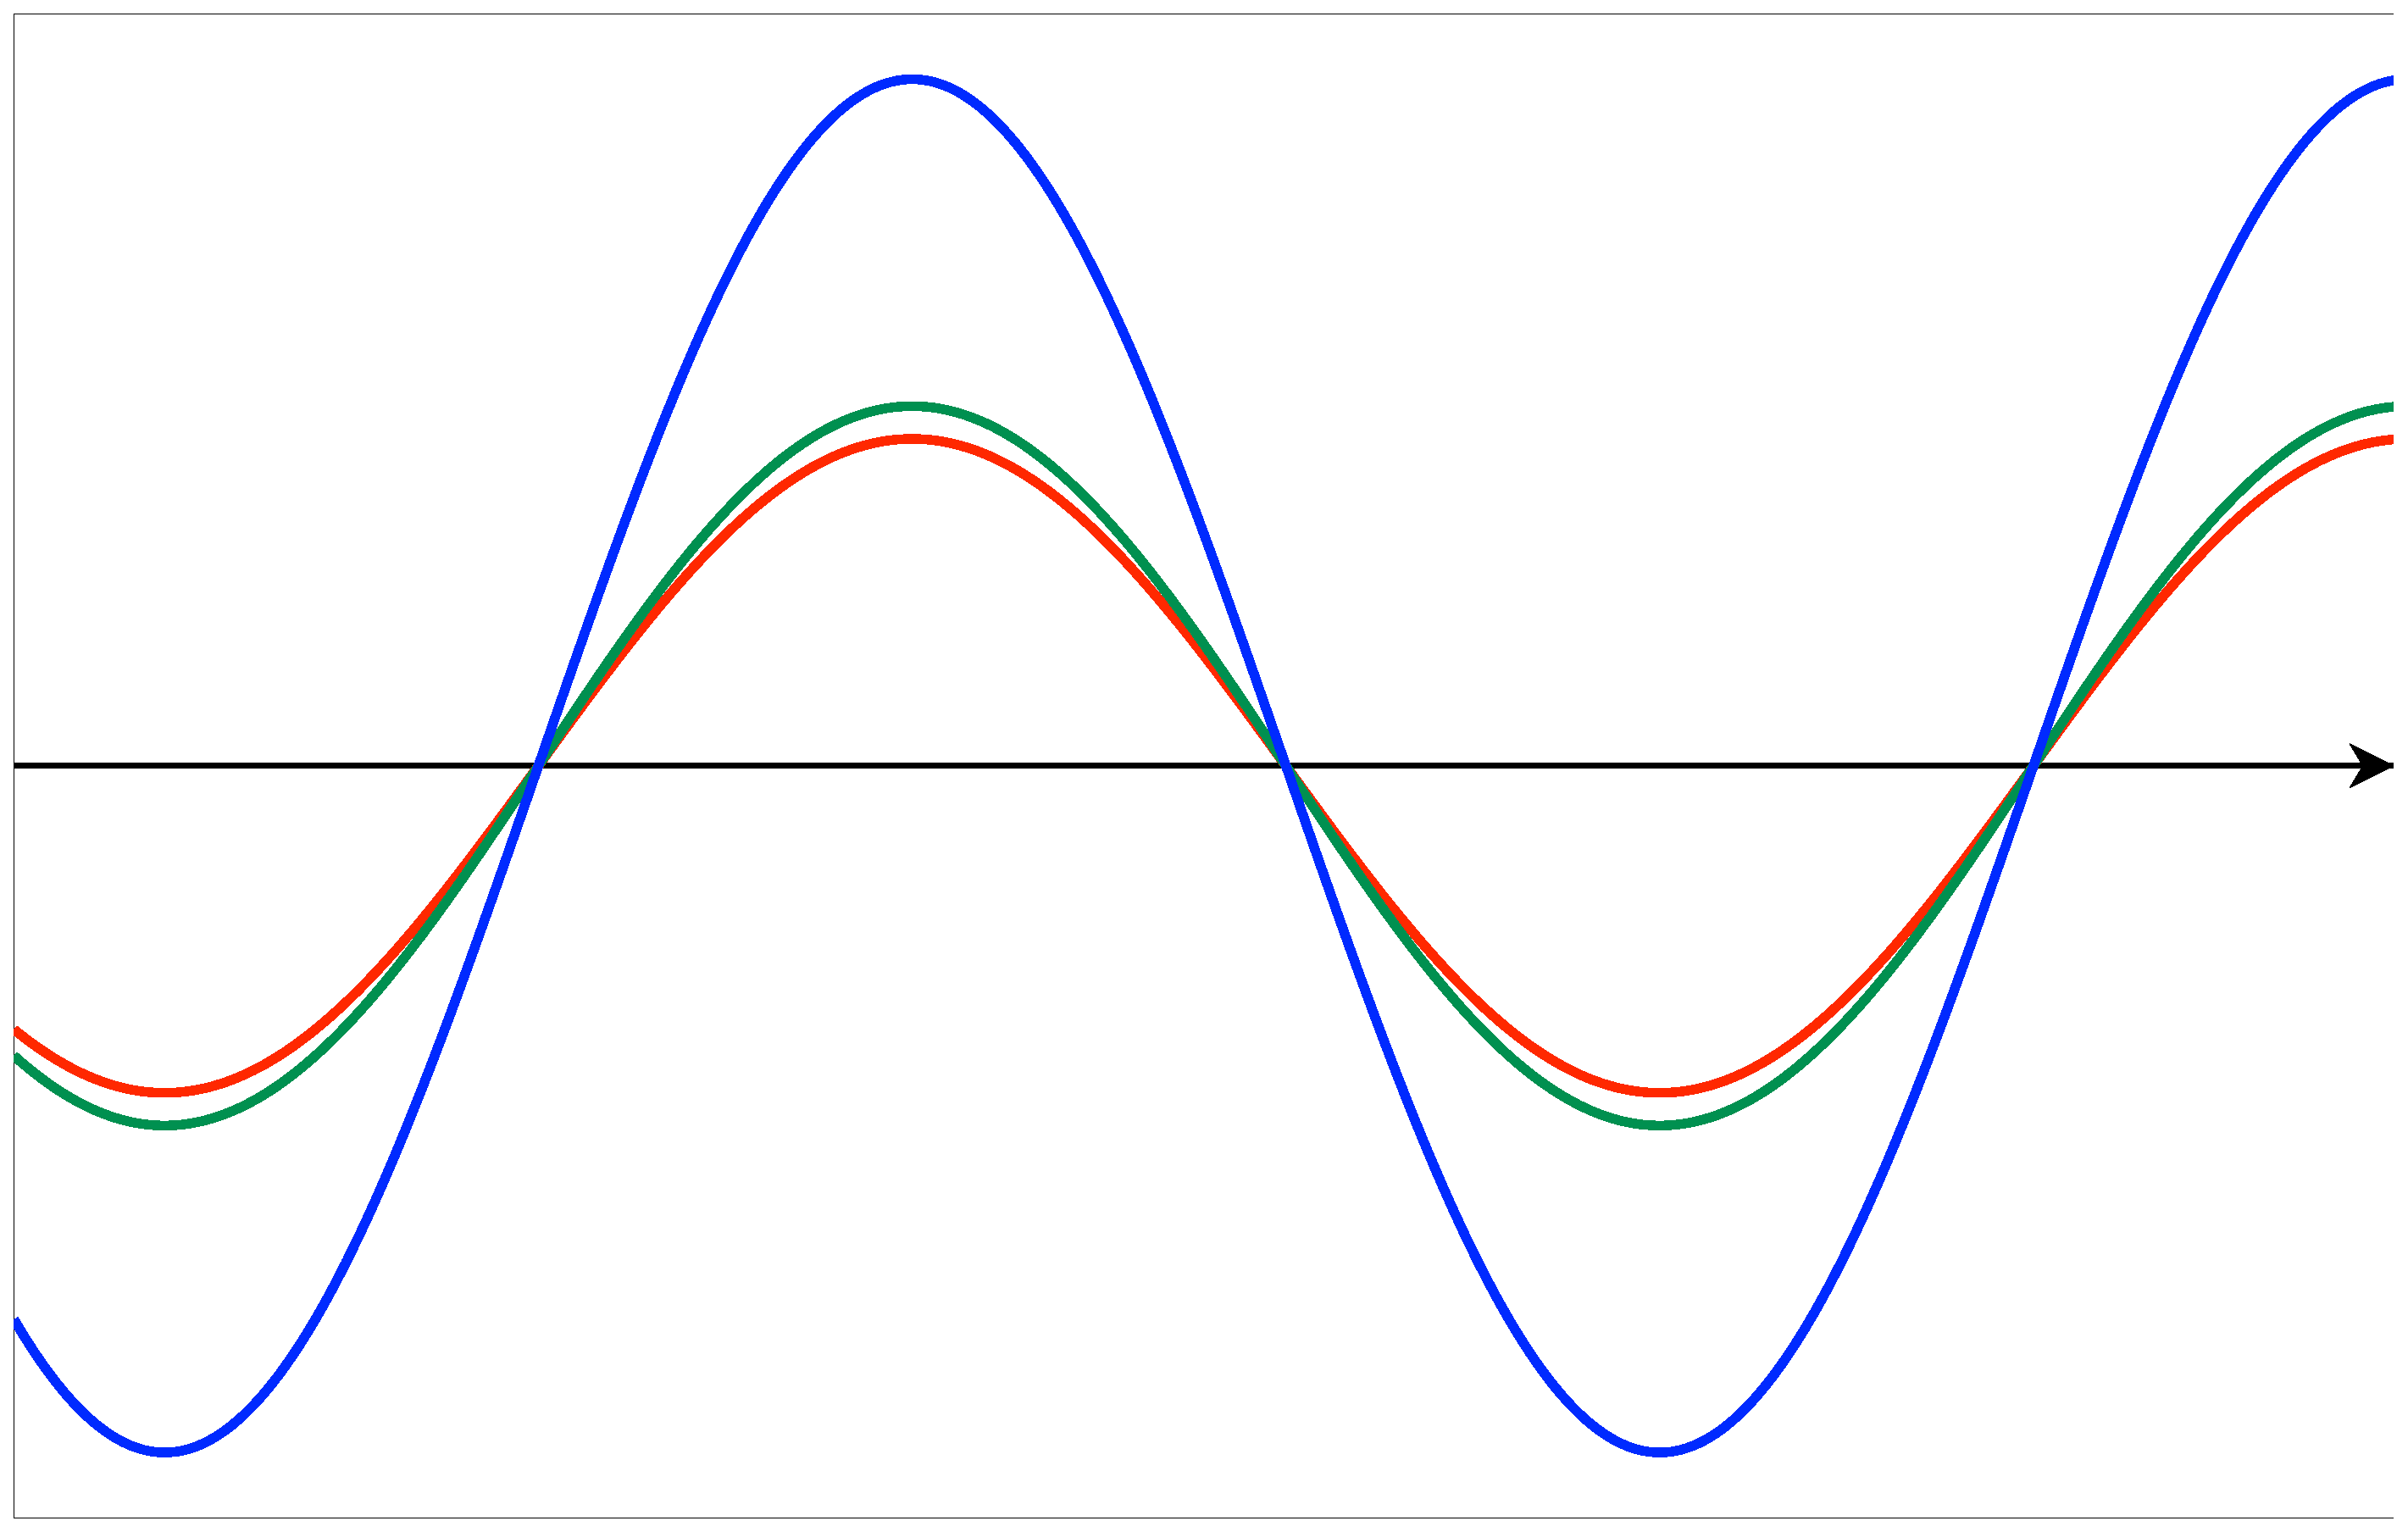
\includegraphics[scale=0.1]{01_Wave/interference3.eps}\\
(A) 強くなる
& (B) 打ち消し合う
& (C) 最も強め合う\\
& (山と谷が合致) & (山と山、谷と谷が合致)
\end{tabular}\\
\bigskip
波の干渉:{\color{red}\maru{1}}+{\color{green}\maru{2}}$\rightarrow${\color{blue}\maru{3}}
\qquad
{\color{red}\maru{1}}の波と{\color{green}\maru{2}}の波が干渉して{\color{blue}\maru{3}}の波ができる
\end{center}

\subsubsection{波の回折}

\begin{wrapfigure}[6]{r}{5.5cm}
\vspace*{-0.8cm}
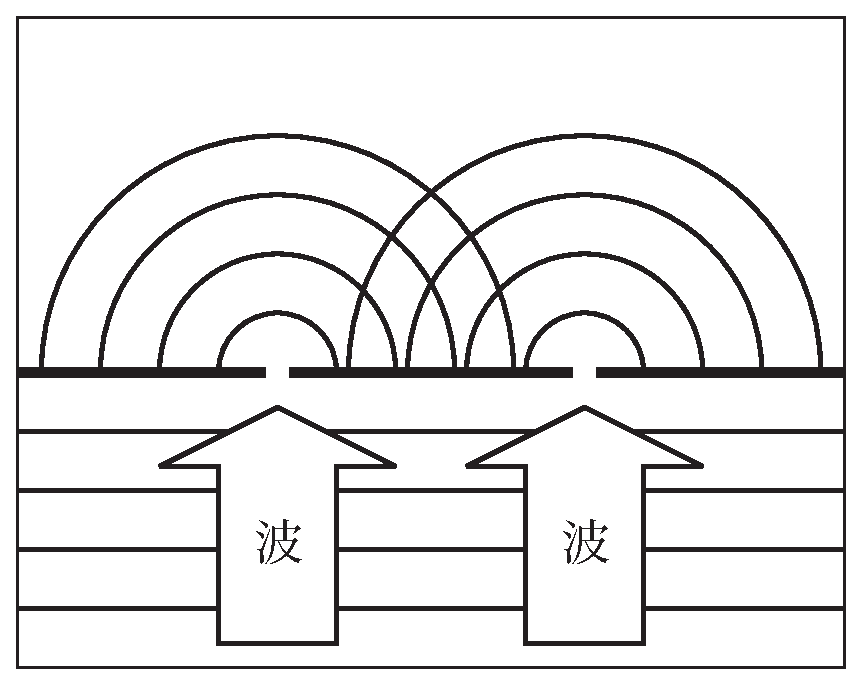
\includegraphics[scale=0.38]{01_Wave/diffraction.eps}
\end{wrapfigure}

進行している波を細いスリットの開いた障壁で遮ると、スリットを通っ
た波は直進せず、スリット上の各点を中心とした球面波を発生し、障壁の裏側まで回り込むよ 
うに伝わります。この現象を波の{\bf 回折}といいます。
スリットの幅に比べて波の波長が大きいほど、回折の程度は大きくなります。
($\Leftrightarrow$波長と比べてスリットの幅がかなり大きければ、回折は起こらず波は直進します。)

\subsection{ドップラー効果と衝撃波}

波が発生している場所(波源)が移動しているとき、進行方向の前方の波長は短く詰まり周波数が高くなり、
後方の波長は長く伸び周波数は低くなります。
この現象のことを{\bf ドップラー効果}と言います。

静止している観測者に向かって伝播速度$V$、振動数$\nu$の波の波源が速度$v$で同一直線上を移動しているとき、
観測者が受ける波の振動数$\nu'$は
\[
\nu' = \nu \times \frac{V}{V-v}
\]
となります。ただし、$v$は観測者に向かう向きを正とし、遠ざかるときは負とします。

この式を見ると、波源の移動速度が波の伝播速度$V$と等しくなったとき、波源の移動方向前方
の波は圧縮され振動数は無限大になります。このとき波源の先頭で重なりあった強い波を{\bf 衝撃波}
と言います。一般に波源の移動速度が波の伝播速度を上回ったとき衝撃波が発生します。

音速を超えて飛行するジェット機などの周囲にも衝撃波が発生し、
その衝撃波が大音響として聞こえることもあります。

\subsection{水深と波の速度}

水面で発生する波の場合、その波の高さや水深によって波の進行速度が変わります。波の高さを$h$、水深を$d$、
重力加速度を$g(=9.8\, [{\rm m/s}^2])$とすると、水波の進行速度は近似的に
\[
v = \sqrt{g(h+d)}
\]
で与えられます。この式から、水深の深い海の中心部よりも水深の浅い沿岸部の方が波の速度が遅くなる
ということがわかります。

\newpage

\jikken

\begin{itemsquarebox}[c]{\bf 実験用具}
水波投影装置、水波発生器(空圧式)、水波発生装置(磁石式)、アクリルブロック、消しゴム、カメラ機能付きスマートフォン(デジタルカメラ)
\end{itemsquarebox}

\bigskip

\subjikken{水波の観察}

\begin{enumerate}

\item 水槽に水を張り、ランプを点灯させます。

\item 水波発生器(空圧式)に単波用ノズル(L字型)を取り付けます。

\item 水波発生器(空圧式)のスイッチを入れ、ノズルの先端を水面に近づけ噴射量の調整をします。

\item ランプの光の角度等を水波が観察しやすいように調節します。

\item アクリルブロックや消しゴム等でスリットを作り、水波がスリットを通ったときの波の回折の様子を観察しましょう。水波はスマートフォン等でスロー動画撮影して記録すると観察が容易になり、水波の伝わる様子がよくわかります。

\item ノズルの先と水面との距離を一定に保ち、波源を一方向に動かします。
そのときの水波の様子をスマートフォン等で撮影し、観察します。波源の進行方向と
その反対側で水波の形状(波長)はどうなっているでしょうか? $\Rightarrow$ドップラー効果

\item 波源の移動速度をさらに速くし、水波の速度を超えると水波の形状はどうなるでしょうか? $\Rightarrow$衝撃波面の形成

\item 水波発生装置(磁石式)を水槽の縁に取り付け、振動片先端が水面に接するようにします。

\item 水波発生装置(磁石式)のスイッチを入れ、ダイアルで振動周波数の調整をします。
(ダイアルを最大にしてから始動させます。)

\item 2つの波源から出た水波が強め合ったり、弱め合ったりする時の水波の形状を観察します。 $\Rightarrow$波の干渉

%\item バットにプラスチック板を斜めにして沈め、そこにぶつかった水波の様子を観察しましょう。
%水深と波長の間に何か関係があるでしょうか? また、その関係から何がわかるでしょうか?

\end{enumerate}

%※ デジタルカメラはストラップなどを手に巻き付けるなどしてしっかり固定し、水を入れたバットに落としたりしないよう注意して操作しましょう。


